\documentclass[sigconf,nonacm]{acmart}

\usepackage{booktabs}
\usepackage{array}

\newcommand{\preset}[1]{\textit{#1}}

\copyrightyear{2027}
\acmYear{2027}
\setcopyright{cc}
\setcctype{by}
\acmConference[NIME '27]{International Conference on New Interfaces for Musical Expression}{2027}{}

\title{\texorpdfstring{\vspace*{-50pt}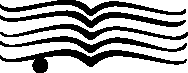
\includegraphics[width=0.15\linewidth]{Assets/logo.pdf}\\[4pt]}{}REMORA: Real-time Expressive Motion Routing for Audio}

\author{Timothée Dravet}
\affiliation{%
  \institution{Polytech Marseille, Aix-Marseille Université}
  \country{France}
}
\email{timothee.dravet@etu.univ-amu.fr}

\author{Daniel Overholt}
\affiliation{%
  \institution{CREATE, Aalborg University}
  \country{Denmark}
}
\email{dano@create.aau.dk}

\renewcommand{\shorttitle}{}
\renewcommand{\shortauthors}{}

\begin{document}

\begin{abstract}
REMORA turns a martial-arts staff (b\^o) into a musical instrument. A wireless inertial sensor on
the staff streams its orientation and motion to an audio plugin, where spins, changes of facing,
and thrusts become sound in real time. The b\^o is a full-length, two-handed, swung object with its
own rotational inertia and an established movement vocabulary, and we derive features specific to
it: the plane and direction of a spin, a coarse facing that needs no magnetometer, a lap counter,
and an axial thrust detector. The gesture-to-sound mapping is a small dataflow patch that the
performer can see and rewire on a canvas inside the plugin while it plays. We describe the
hardware, a user-guided calibration that makes the instrument independent of how the sensor is
rotated on the staff, the motion features, and the mapping layer, and we discuss how common b\^o
techniques relate to the presets. A pilot session with ten first-time players found the instrument
comfortable and engaging, and identified thrust detection as its main defect, for which we give a
probable cause.
\end{abstract}

\begin{CCSXML}
<ccs2012>
<concept>
<concept_id>10010405.10010496</concept_id>
<concept_desc>Applied computing~Sound and music computing</concept_desc>
<concept_significance>500</concept_significance>
</concept>
<concept>
<concept_id>10011007.10011006.10011050.10011058</concept_id>
<concept_desc>Software and its engineering~Visual languages</concept_desc>
<concept_significance>300</concept_significance>
</concept>
</ccs2012>
\end{CCSXML}
\ccsdesc[500]{Applied computing~Sound and music computing}
\ccsdesc[300]{Software and its engineering~Visual languages}
\makeatletter
\renewcommand\@concepts{%
  \textbullet\ \textbf{Applied computing} \textrightarrow\ \textbf{Sound and music computing};\\
  \textbullet\ \textbf{Software and its engineering} \textrightarrow\ \textit{Visual languages}.}
\makeatother

\keywords{digital musical instrument, martial arts, b\^o staff, inertial sensing, gesture mapping,
visual patching, OSC}

\begin{teaserfigure}
  \centering
  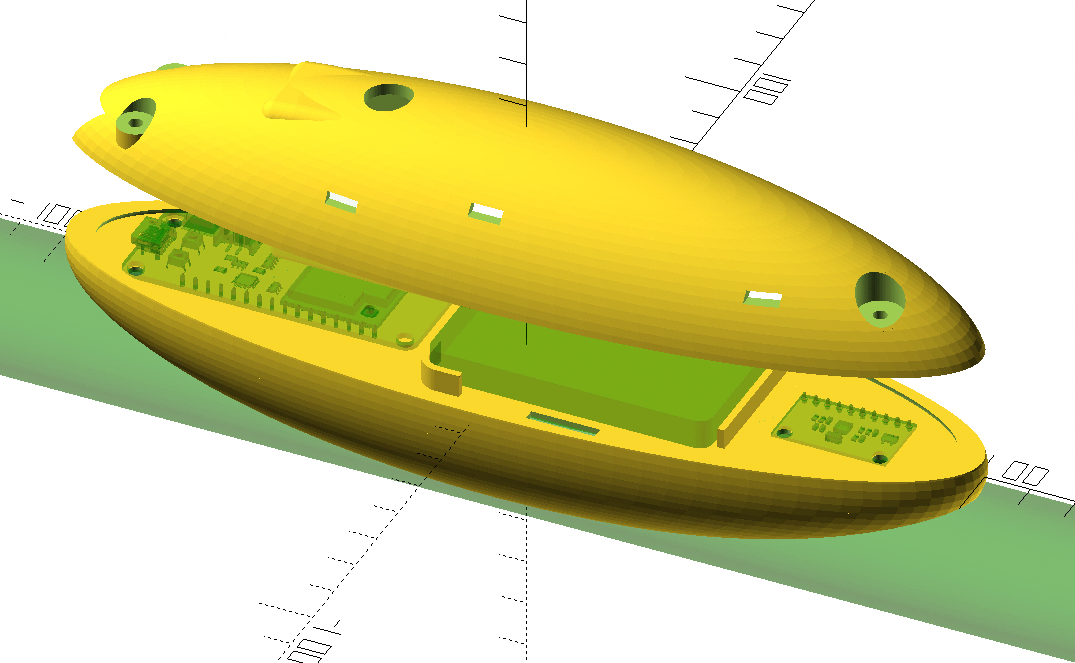
\includegraphics[height=4.2cm]{Assets/openscad_casing.png}\hspace{1em}
  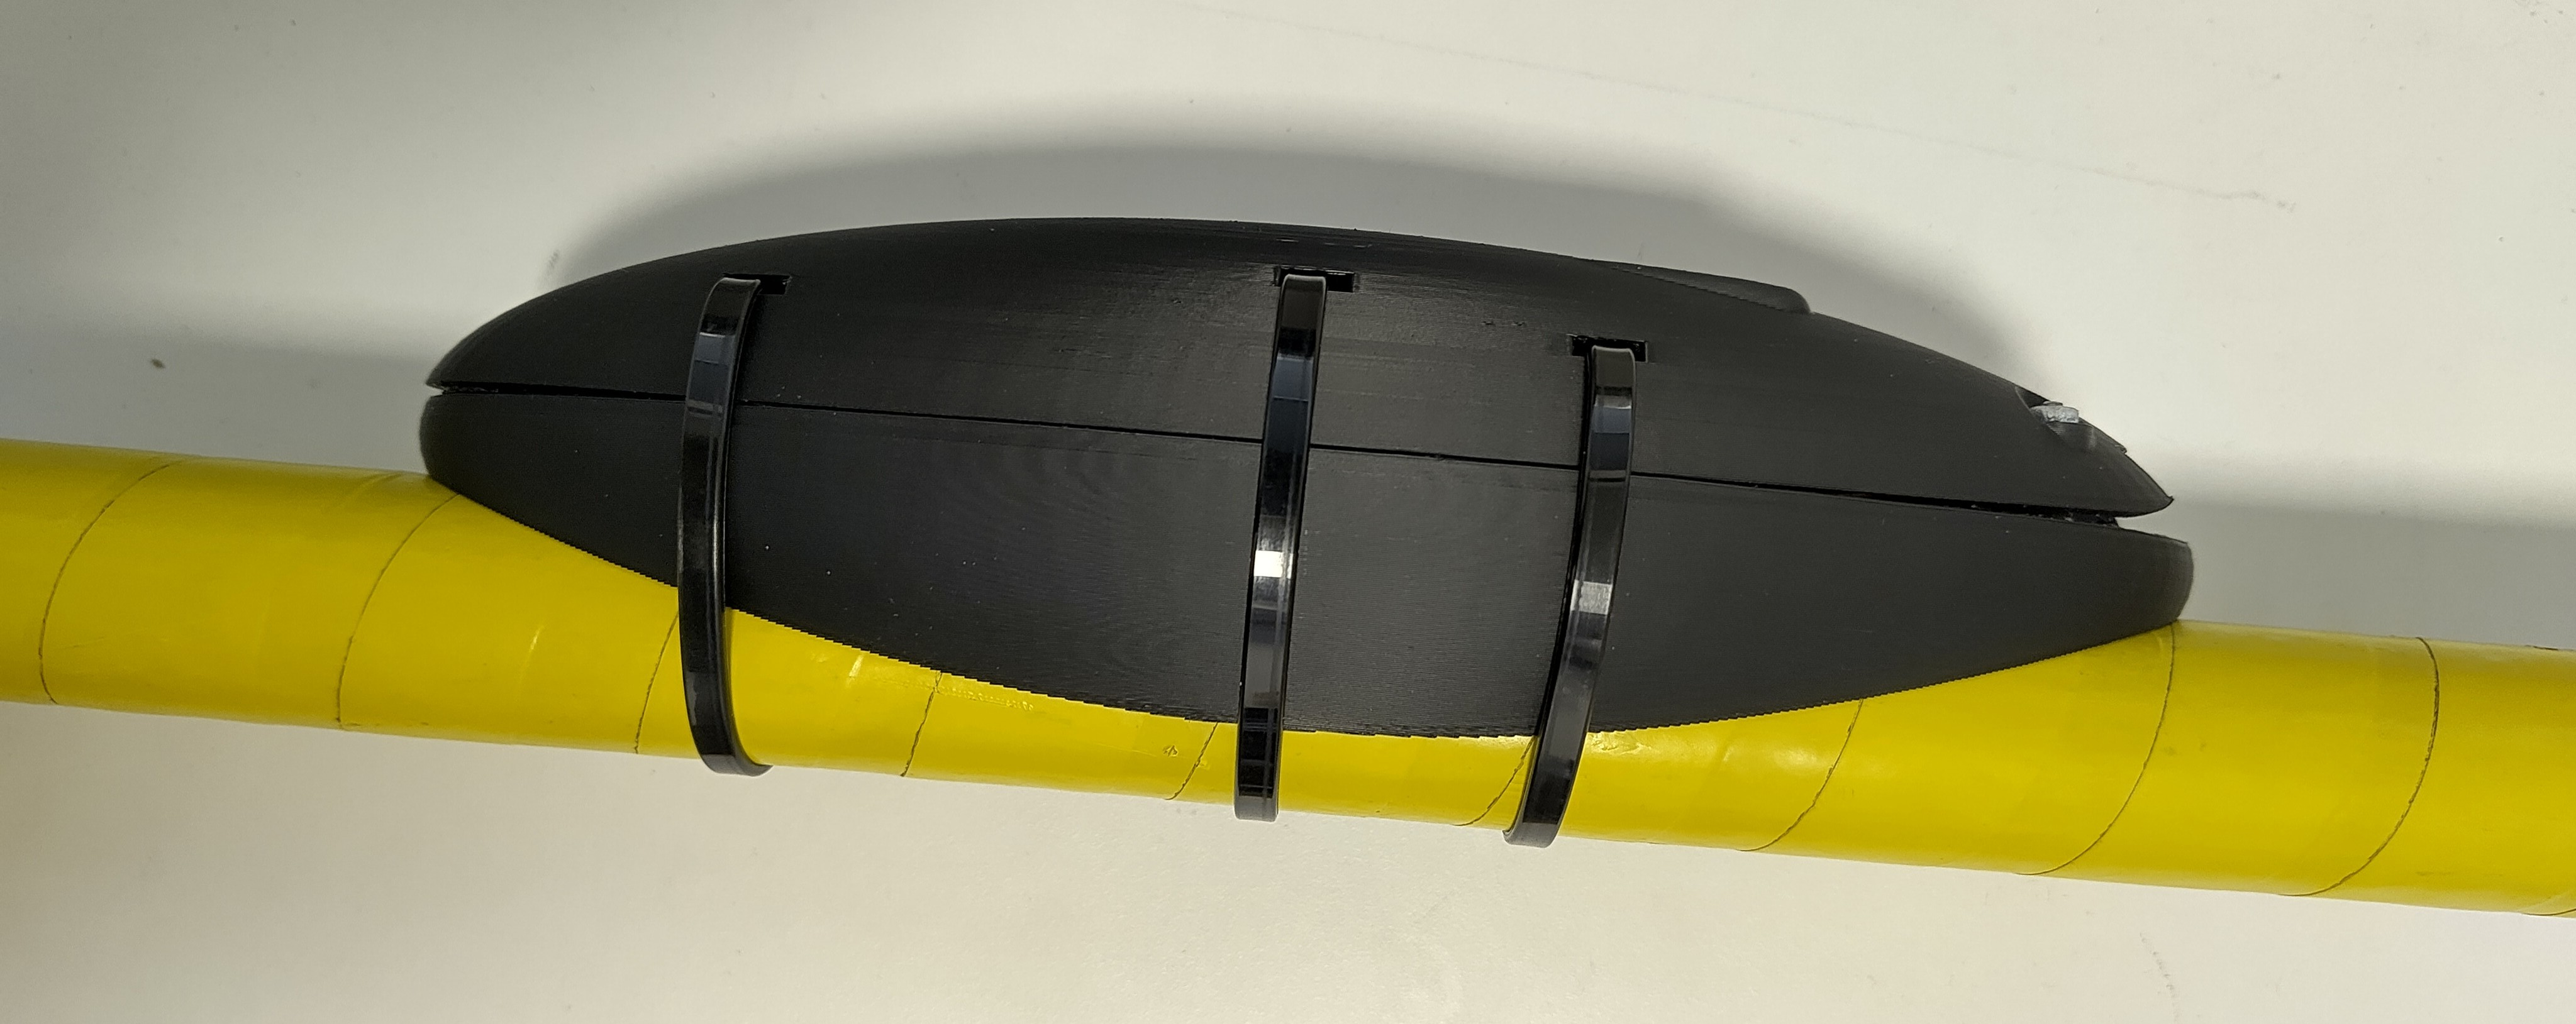
\includegraphics[height=4.2cm]{Assets/casing_on_staff.jpg}
  % TODO (authors): replace or complement with a photo of the staff being played.
  \caption{The REMORA sensor unit: parametric OpenSCAD enclosure (left) and the printed enclosure
  zip-tied near one end of the b\^o (right).}
  \label{fig:enclosure}
\end{teaserfigure}

\maketitle

\section{Introduction}

\subsection{Motivation}
REMORA comes from the first author's practice in both martial arts and music. The b\^o is a staff of
about 1.5\,m, held in two hands and swung, spun, and thrust through a body of techniques that are
taught as forms (\emph{kata}). Inertial-sensor Digital Musical Instruments (DMIs) presented at New
Interfaces for Musical Expression (NIME) are mostly small handheld or body-worn objects. A b\^o
instead brings a full-body object, rotational inertia, reach, and an existing gesture vocabulary
that a trained performer already controls precisely.

Finding a gesture vocabulary for such an object took many attempts. At first each gesture-to-sound
mapping was its own code module, and every change meant a rebuild. After eleven of them, we moved
the mapping into a small dataflow patch that is edited live inside the audio plugin that makes the
sound. Visual patching is well established (\S\ref{sec:related}); in REMORA it is the tool for
writing and revising the staff's vocabulary.

\subsection{Contributions}
This paper describes a working instrument and a first pilot study. Its contributions are:
\begin{enumerate}
\item \label{claim:features} A b\^o-staff instrument whose motion features are specific to a long
swung object: spin plane and direction, a coarse facing derived without a magnetometer, a
continuous lap count, and an axial thrust detector (\S\ref{sec:features}).
\item \label{claim:calibration} A two-stage, user-guided calibration that removes the effect of how
the sensor is rotated on the staff (\S\ref{sec:calibration}).
\item \label{claim:dag} A mapping layer inside the plugin, built as a typed directed acyclic graph
(DAG) that the performer can rewire while audio runs (\S\ref{sec:mapping-arch}).
\item \label{claim:presets} Fifteen presets built from one catalog of 69 node types, from a
two-control starter mapping to spin- and facing-driven mappings for trained players
(\S\ref{sec:named-mappings}).
\end{enumerate}
Table~\ref{tab:claims-evidence} sets out the evidence for each contribution and what remains
untested.

\subsection{Scope}
The intended performer is a soloist with some staff or martial-arts background, playing a set built
from presets. The catalog is graded: \preset{Simple} needs only tilt and roll, while the facing- and
spin-driven \preset{Martial Momentum} and \preset{Azimut Kinetic} reward b\^o technique. Because
the mapping is a patch, REMORA may also interest patch-based electronic musicians looking for a
full-body controller. Ensemble use is out of scope.

\section{Related Work}
\label{sec:related}

\subsection{Rod, Baton, and Swung Controllers}
The \textit{T-Stick}~\cite{malloch2007tstick} senses touch and pressure along its shaft together
with accelerometer-derived shake and tap gestures. Conducting interfaces include Mathews'
\textit{Radio Baton}~\cite{mathews1991radiobaton}, Marrin and Paradiso's \textit{Digital
Baton}~\cite{marrin1997digitalbaton}, and the \textit{Conductor's
Jacket}~\cite{marrin1998conductorsjacket}. Nam's \textit{mPoi}~\cite{nam2013mpoi} established swung
objects as a DMI form, and \textit{x-OSC}~\cite{madgwick2013xosc} popularised the Wi-Fi/OSC inertial
streaming pattern that REMORA's sensor unit follows.

\subsection{Mapping Tools and Visual Patching}
Visual dataflow patching descends from Puckette's Patcher, now
\textit{Max}~\cite{puckette1988patcher,puckette2002maxatseventeen}, and continues in \textit{Pure
Data}~\cite{puckette1996puredata} and \textit{VCV Rack}~\cite{belt2017vcvrack}. For DMIs,
libmapper~\cite{malloch2015libmapper} and its graphical front end
Webmapper~\cite{wang2019webmapper} connect controller signals to synthesis parameters across a
network, and \textit{ossia score}~\cite{celerier2015ossia} combines such mappings with a timeline.
Any of these could host REMORA's mappings. We put the graph inside the plugin for practical
reasons: mapping and synthesis share one process and one preset file, and the patch shows each
signal's live value next to the synth it drives (\S\ref{sec:live-patching}). The closest prior
system is the T-Stick with libmapper. REMORA differs in its controller and features: a full-length
swung b\^o has a spin plane, a spin direction, and a facing, for which a handheld rod's touch and
shake gestures have no counterpart.

\subsection{Mapping Strategies}
Hunt and Wanderley~\cite{hunt2002mapping} classify mappings as one-to-one, one-to-many, or
many-to-one, and argue that richer mappings make an interface feel like an instrument. Van Nort et
al.~\cite{vannort2014mapping} extend mapping to continuous navigation between parameter spaces;
REMORA's graph stays with explicit parameter-level functions. \textit{Wekinator}~\cite{fiebrink2010wekinator}
and Fran\c{c}oise et al.~\cite{francoise2014probabilistic} learn mappings from example gestures
instead of having the performer wire them.

Expressive-movement systems often describe motion with Laban's Effort
factors~\cite{camurri2000eyesweb,schacher2010motiontogesture}, and Fdili Alaoui et
al.~\cite{fdilialaoui2017laban} show that capturing them well takes expert annotation and
multimodal data. REMORA uses simpler kinematic signals tied to the staff (\S\ref{sec:features}).

\section{Design}
Five requirements shaped the design:
\begin{itemize}
\item \textbf{A real b\^o.} The instrument keeps the reach, weight, and two-handed grip of a
full-length staff.
\item \textbf{Wireless during performance.} A cable is acceptable only for charging.
\item \textbf{Live-editable mapping.} Loading or rewiring a mapping must not interrupt audio.
\item \textbf{Mount-agnostic calibration.} Behaviour should not depend on exactly how the sensor is
strapped to the staff.
\item \textbf{Low latency.} The sound should follow the motion closely enough to feel driven by it
(\S\ref{sec:latency}).
\end{itemize}
The firmware samples the Inertial Measurement Unit (IMU) and sends Open Sound Control (OSC) packets
over Wi-Fi. The plugin does everything downstream: OSC reception, calibration, motion analysis,
graph evaluation, and synthesis.

\section{Implementation}

\subsection{Hardware}
\label{sec:build}
The sensor unit is a SparkFun ESP32-S2 Thing Plus reading an MPU-9250 IMU over I2C at 400\,kHz,
powered by a 2000\,mAh LiPo battery (Figure~\ref{fig:hardware}). It sits in a parametric OpenSCAD
enclosure sized to the staff diameter (Figure~\ref{fig:enclosure}) and is attached near one end, out
of the performer's grip, with zip ties, so it can be moved or removed without damaging the staff.
Because calibration absorbs the sensor's rotation, the enclosure can be strapped on at any angle.
Its position along the staff does matter (\S\ref{sec:features}) and should be kept constant between
sessions.

Orientation is estimated on the microcontroller by the \texttt{hideakitai/MPU9250} library (v0.4.8)
with its Mahony filter, which fuses accelerometer and gyroscope only; the magnetometer is not used
(\S\ref{sec:limitations}). The library's default ranges ($\pm16$\,g, $\pm2000^\circ$/s) are kept;
fast spins approach the gyroscope limit. Each OSC packet carries the quaternion, raw acceleration,
angular rate, and magnetic field, and is sent over UDP at most once every 10\,ms (nominally
100\,Hz). The host computer runs a Wi-Fi hotspot and the staff joins it directly, so no separate
access point is needed.

\begin{figure}[htbp]
  \centering
  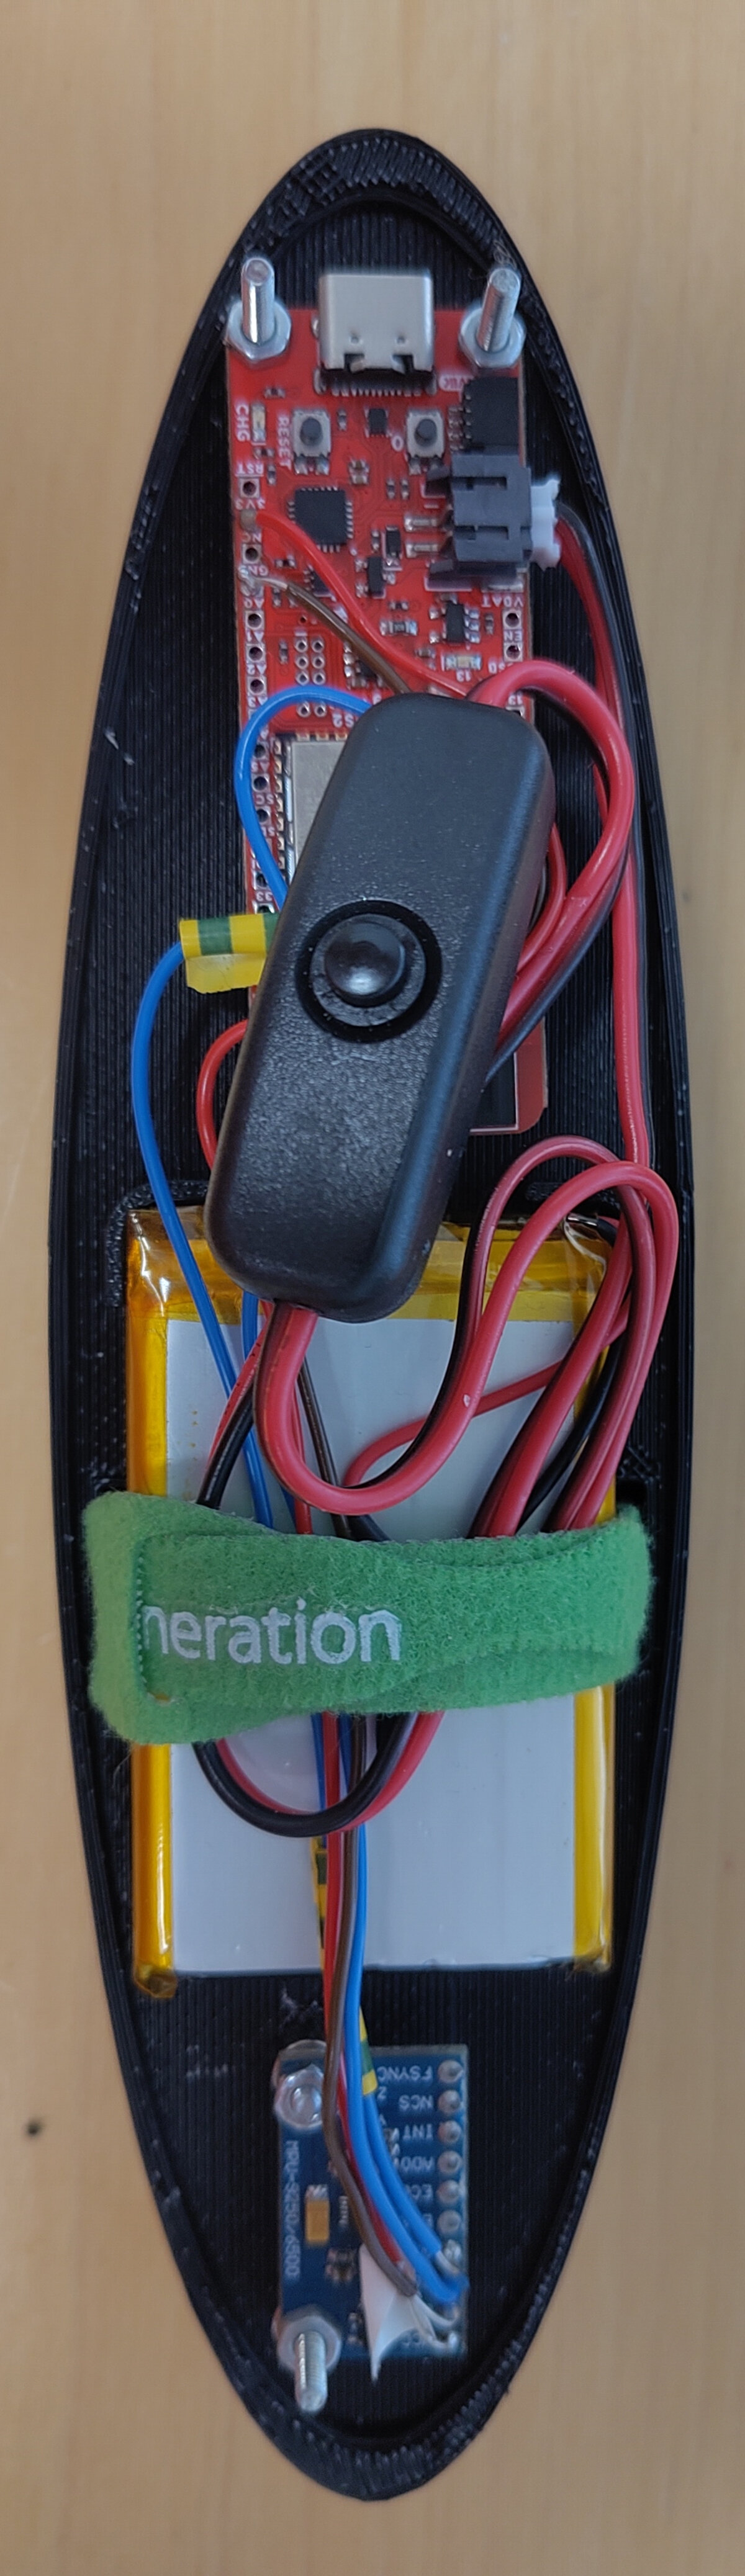
\includegraphics[angle=270, width=0.55\linewidth]{Assets/hardware_wiring.jpg}
  \caption{Inside the enclosure: ESP32-S2, MPU-9250 IMU, and LiPo battery.}
  \label{fig:hardware}
\end{figure}

\subsection{Calibration}
\label{sec:calibration}
Orientation is tracked as a unit quaternion; rotating $v$ by $q$ gives $v' = q\,v\,q^{-1}$. The
performer is prompted through three poses, in order: $A$, staff horizontal pointing forward; $B$,
staff vertical pointing up; $C$, staff horizontal pointing right (quaternions $q_A,q_B,q_C$).

\textbf{Stage 1: which sensor axis runs along the staff.} Each candidate axis
$L \in \{\pm X, \pm Y, \pm Z\}$ is scored by
\[
v_P = \widehat{\mathrm{rotate}(L, q_P)}\,,\qquad e(L) = |v_A{\cdot}v_B| + |v_B{\cdot}v_C| +
|v_C{\cdot}v_A|\,.
\]
Only the staff axis is carried through three mutually orthogonal directions by the three poses, so
it has the lowest $e(L)$. $L$ and $-L$ score the same but give opposite signs of the triple product
$(v_A \times v_B)\cdot v_C$. Which sign marks the tip depends on the IMU library's frame
convention; with the library we use, it is the negative one:
\[
L^\ast = \operatorname*{arg\,min}_{L\,:\,(v_A \times v_B)\cdot v_C < 0} e(L)\,,
\]
which gives the alignment quaternion $q_{\text{align}}$. If the poses are too close together or
nearly coplanar, calibration is rejected and the performer is asked to retry.

\textbf{Stage 2: heading and twist.} From the measured staff axis in poses $A$ and $B$ ($b_0$,
$b_1$), an orthonormal triad $U = [\,b_0,\ \widehat{b_0\times b_1},\
b_0\times\widehat{b_0\times b_1}\,]$ is built, and likewise $W$ from the instrument-frame forward
$(1,0,0)$ and up $(0,0,1)$. The aligning rotation is the orthogonal-Procrustes solution
$R = W U^{\top}$, converted to a quaternion $q_{\text{corr}}$. Every reading is then mapped to
instrument space by $q' = q_{\text{corr}}\,(q_{\text{raw}}\,q_{\text{align}})$, whatever the
sensor's rotation on the staff. Its position along the staff is not corrected
(\S\ref{sec:limitations}).

\subsection{Motion Features}
\label{sec:features}
A single motion analyzer computes the features in Table~\ref{tab:motion-features}, and every
mapping graph reads from it. It currently runs once per audio block on the latest sensor packet,
with $\Delta t$ from the host clock (\S\ref{sec:limitations}). All smoothing rates and thresholds
below were tuned by ear on the instrument, at one host buffer size.

\begin{table}[htbp]
\centering
\small
\caption{Motion features computed by the analyzer.}
\label{tab:motion-features}
\begin{tabular}{@{}p{0.34\linewidth}p{0.58\linewidth}@{}}
\toprule
Feature & Purpose \\
\midrule
Tip vector, rotation axis & tip velocity and spin axis \\
Dynamic acceleration & motion with gravity removed \\
Energy, onset, axis stability, jerk & how hard and how steadily the staff moves \\
Spin plane and direction & vertical/horizontal spin, CW/CCW \\
Facing & which horizontal axis the staff aligns with \\
Continuous spin count & full turns in the current spin \\
Axial thrust & stab or strike along the staff \\
\bottomrule
\end{tabular}
\end{table}

\textbf{Tip, axis, and gravity.} The tip direction $p_n = \mathrm{rotate}((1,0,0), q_n)$ is kept
over three samples to estimate tip velocity and the current rotation axis. Gravity is estimated by
smoothing the inverse-rotated world $+Z$ axis with a one-pole filter ($\alpha{=}0.10$), and
subtracted from the raw reading to give the dynamic acceleration $a_{\text{dyn}}$.

\textbf{Energy features.} Four smoothed signals describe how hard the staff is moving. Each applies
the one-pole smoother $y_n = y_{n-1} + \alpha\,(x_n - y_{n-1})$ to a derivative of
$a_{\text{dyn}}$ or of gyroscope magnitude. \emph{Energy} is the enveloped magnitude of a leaky
integral of $a_{\text{dyn}}$. \emph{Onset} is the positive rate of change of gyroscope magnitude.
\emph{Axis stability} is the smoothed absolute dot product between consecutive rotation axes, high
when the staff keeps spinning around the same axis. \emph{Jerk} is the smoothed jerk of
$|a_{\text{dyn}}|$, split into smooth and abrupt parts. (In the source code these four are named
after Laban's Effort factors: Weight, Time, Space, and Flow.) With the unit near the tip, the
sensor sits about $r \approx 0.7$\,m from the centre of rotation, and a 2\,rev/s spin produces a
centripetal acceleration $\omega^2 r \approx 11$\,g. This term dominates $a_{\text{dyn}}$, so
Energy and Jerk mainly follow spin speed, which is how the presets use them, and their scale
changes if the unit is moved along the staff.

\textbf{Spin plane and direction.} Let $(a_x,a_y,a_z)$ be the rotation axis, smoothed with
$\alpha{=}0.35$. The spin is classified as \emph{vertical} (the staff turns in a vertical plane,
like a baton twirled beside the body) when
\[
\sqrt{a_x^2 + a_y^2} > |a_z|\,,
\]
and as \emph{horizontal} (like a propeller overhead) otherwise. For a horizontal spin, the direction
is the sign of $a_z$. For a vertical spin, it is the sign of the larger of $a_x, a_y$, or, in the
\preset{Martial} presets, the sign of the axis' dot product with a reference axis latched at the
first vertical spin after the preset loads.

\textbf{Facing.} A compass heading would need the magnetometer, which is unreliable next to the
staff's electronics and stage equipment. REMORA instead asks which horizontal axis of the calibrated
frame the staff is closer to: $x$ (the calibration ``forward'', labelled \emph{north}) or $y$
(\emph{east}). Let $(d_x,d_y)$ be the horizontal components of the rotation axis during vertical
spins, or of the tip direction otherwise. With hysteresis factor $k = 1.15$, the state switches
\[
\text{north}\rightarrow\text{east if } |d_y| > k\,|d_x|\,,\qquad
\text{east}\rightarrow\text{north if } |d_x| > k\,|d_y|\,.
\]
Measured from the $x$ axis, the switch points are therefore $\arctan(1.15) \approx 49^\circ$ and
$\arctan(1/1.15) \approx 41^\circ$, which prevents flicker at the boundary. Because orientation is
6-axis, heading is relative to the calibration pose and drifts with gyroscope yaw
(\S\ref{sec:limitations}).

\textbf{Continuous spin count.} $\lVert\omega\rVert\,\Delta t$ is accumulated, and a lap is counted
every $360^\circ$; the count resets when the spin plane or direction changes.

\textbf{Axial thrust.} A thrust is flagged when the jerk of the dynamic acceleration projected on
the staff axis crosses zero while its magnitude exceeds $1.5$\,g, gated to slow rotation
($\lVert\omega\rVert < 90^\circ$/s) and followed by a cooldown.

\subsection{Mapping Architecture}
\label{sec:mapping-arch}
The node catalog has four categories: Source (sensor values and the features above), Math, Sink
(one node per synthesis engine exposing all its parameters as typed inputs, plus output gain), and
Display (live monitors). A graph is a set of nodes plus typed wires, saved as an XML preset. The
graph is the only path from sensor to synthesiser.

When a wire is added, the graph recomputes a topological order with Kahn's algorithm and refuses
the wire if it would close a cycle. Each audio block, evaluation walks the cached order once and
every node computes
$y_i = f_{\text{type}(n_i)}(x_{i,1},\dots,x_{i,m};\theta_i)$ from its inputs $x$ and parameters
$\theta$. The patch is thus one composed function of the sensor frame, with no sorting on the audio
thread. If the user interface is editing the graph when a block arrives, evaluation does not wait;
it reuses the previous block's output.

Math nodes cover arithmetic, shaping (linear and logarithmic range mapping, clamp, threshold,
crossfade, quantise, sine, atan2, semitones to Hz), lookup tables (1-D, and an 8-entry table indexed
by three booleans), and stateful dynamics (one-pole smoother, leaky integrator, retrigger envelope,
hysteresis, derivative, latch, random sample-and-hold).

\subsection{Presets}
\label{sec:named-mappings}
The eleven C++ mappings from development were rebuilt as graph presets: \preset{Simple},
\preset{Lead+Drone}, \preset{Spin Filter}, \preset{Bowed Chord}, four \preset{Azimut} variants,
\preset{Martial Effort}, \preset{Martial Momentum}, \preset{Spin Voices}, and \preset{Speed Gate}.
Four more (\preset{Wind Noise}, \preset{Azimut Kinetic}, \preset{Spin Voices (Scale)},
\preset{Vocal Tract}) were made directly as graphs. Nine presets are offered in the plugin's
selector (Table~\ref{tab:presets}); the others are close variants kept as reference patches.

\begin{table}[htbp]
\centering
\small
\caption{The nine presets in the plugin's selector.}
\label{tab:presets}
\begin{tabular}{@{}p{0.3\linewidth}p{0.62\linewidth}@{}}
\toprule
Preset & Character \\
\midrule
\preset{Simple} & Pitch from tilt, volume from roll; one sine voice. \\
\preset{Wind Noise} & No pitch; motion energy swells filtered noise into gusts. \\
\preset{Bowed Chord} & Root from tilt; yaw and roll pick the chord; spin speed acts like bow pressure. \\
\preset{Lead+Drone} & Major-scale lead over a 4-voice drone. \\
\preset{Martial Momentum} & Root from spin plane and direction; glide speed from spin momentum. \\
\preset{Azimut Kinetic} & Root from spin and facing; rotation speed drives the whole timbre. \\
\preset{Speed Gate} & Slow: pentatonic melody. Fast: crossfades to the Azimut mapping. \\
\preset{Spin Voices (Scale)} & Roll selects 1 of 4 scale-quantised voices. \\
\preset{Vocal Tract} & Physically modelled voice; jabs add consonant-like bursts. \\
\bottomrule
\end{tabular}
\end{table}

The catalog has 69 node types (33 source, 29 math, 4 sink, 3 display). Presets range from 7 nodes
(\preset{Simple}) to 178 (\preset{Martial Effort}), with a median of 86. Together they use 50 of
the 69 types; most unused types are raw per-axis sensor values. No preset needed a node type of its
own. Since the catalog grew alongside the hand-coded mappings, this shows that it can express them;
mappings designed by someone who did not build the catalog are still to be tried. Per-preset counts
are generated from the code by a tool in the repository.

\begin{figure}[htbp]
  \centering
  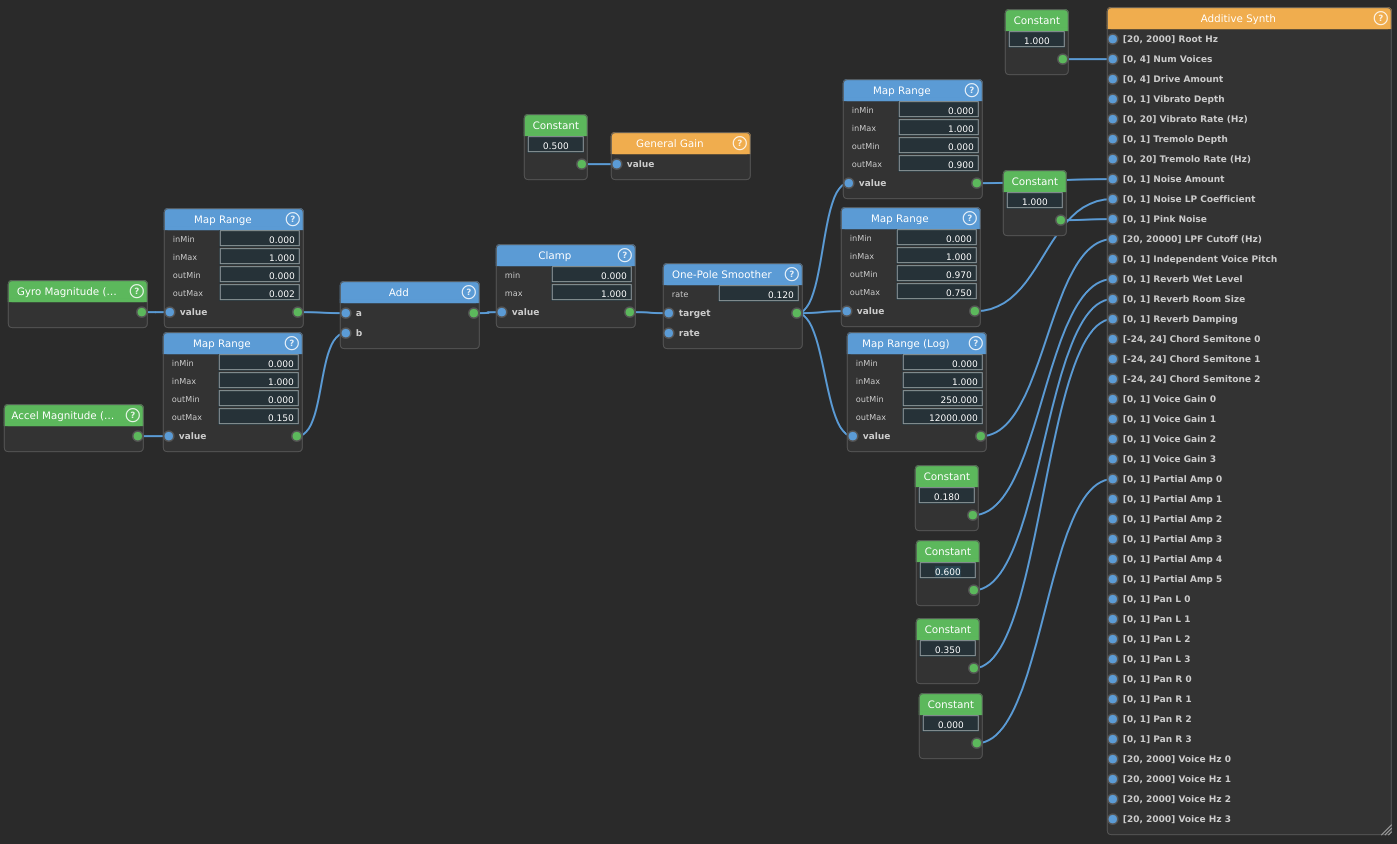
\includegraphics[width=\linewidth]{Assets/wind-noise-preset.png}
  \caption{The complete \preset{Wind Noise} preset in the plugin: gyroscope and acceleration
  magnitudes are scaled, summed, clamped, and smoothed into one motion-energy signal that drives
  the noise level, noise filter, and lowpass cutoff of the additive engine (right).}
  \label{fig:wind-noise}
\end{figure}

\textbf{Azimut root table.} The Azimut presets and the fast branch of \preset{Speed Gate} choose the
root note from three booleans (vertical spin, counter-clockwise, facing east) through the 8-entry
lookup node. The target pitch is reached by a one-pole glide whose rate grows with rotation speed
and jumps at motion onset, so faster motion moves to the new root more quickly
(Figure~\ref{fig:editor}).

\textbf{Kinetic timbre.} \preset{Azimut Kinetic} keeps the Azimut root and maps one smoothed
rotation-energy value $E \in [0,1]$ (gyroscope magnitude normalised over 30--750$^\circ$/s) to many
timbre parameters at once~\cite{hunt2002mapping}: lowpass cutoff, partial amplitudes, drive, noise,
vibrato, tremolo, and reverb. A still staff sounds close to a pure sine; fast spins sound buzzy,
noisy, and reverberant. Each completed lap also triggers a random sample-and-hold, whose values
drift slowly into the same parameters, so two similar spins give two nearby but different timbres.
The whole preset is built from existing math nodes.

\subsection{Live Patching}
\label{sec:live-patching}
The node-graph editor (Figure~\ref{fig:editor}) is a pannable, zoomable canvas. Nodes are coloured
by category, wires are drawn by dragging between typed pins, and new nodes come from a searchable,
categorised picker. Hovering any pin shows its current value, and Display nodes (number, meter,
scope) can be placed on a wire to monitor it. A changed patch can be kept or reverted to its saved
preset in one click, so a mapping can be tried during rehearsal and then kept or dropped.

\begin{figure}[htbp]
  \centering
  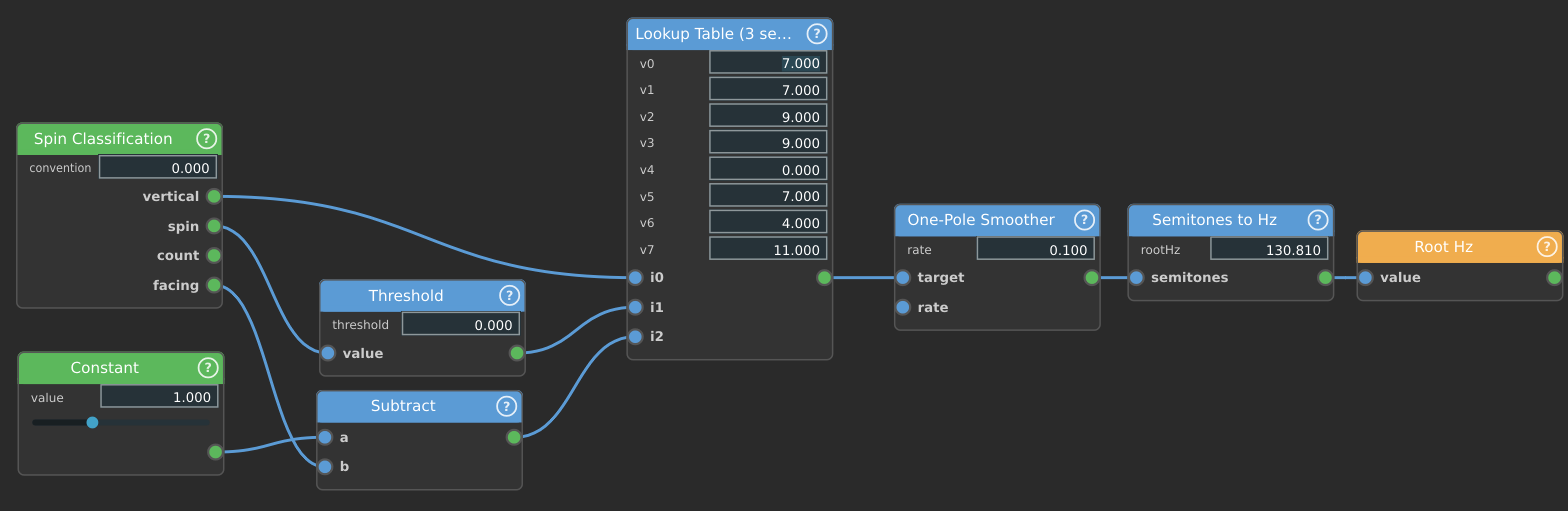
\includegraphics[width=\linewidth]{Assets/node-graph-editor.png}
  \caption{The node-graph editor showing the Azimut root-note chain: spin plane, direction, and
  facing select an entry of the 3-selector lookup table, which is smoothed and converted to the
  root frequency (green Source, blue Math, amber Sink).}
  \label{fig:editor}
\end{figure}

\subsection{Synthesis}
\label{sec:synthesis}
Synthesis engines share one interface and are skipped entirely when the
active preset does not wire them. Every preset except \preset{Vocal Tract} drives the additive
engine: four voices of six harmonic partials, with soft-clip waveshaping, vibrato, tremolo, chorus,
filtered noise, a state-variable lowpass, and reverb. \preset{Vocal Tract} drives a C++ port (via
\texttt{cutelabnyc/pink-trombone-cpp}, MIT-licensed) of Neil Thapen's \textit{Pink
Trombone}~\cite{thapen2017pinktrombone}; only the control layer around it is ours. If no packet
arrives for 150\,ms, the master gain fades out over 120\,ms, and fades back in over 10\,ms when
packets return.

\subsection{Development Iterations}
The graph came last. The first iteration streamed OSC to a minimal receiver with one hard-coded
tilt-to-pitch mapping. The second wrote the mappings as separate C++ classes on top of the shared
analyzer, each adding vocabulary (chords, energy features, facing, thrust). Read side by side, they
were the same arithmetic, shaping, and stateful primitives wired in different patterns, so the third
iteration replaced the classes with the graph engine. Since then, a second synthesis engine
(\S\ref{sec:synthesis}) and four new presets have been added without changes to the engine.

\section{Playing the B\^o: From Technique to Sound}
\label{sec:technique}
The staff-specific features were designed around families of b\^o technique, and this is where the
presets differ most from a generic motion controller.
% TODO (authors): ground this section in your own practice: name the style and the kata or
% drills you use, describe a short performance or étude, and say what playing a familiar form
% through REMORA felt like.

\textbf{Spins.} Two-handed spins beside the body and overhead spins are the staff's most
characteristic motions. Spin plane and direction select among four roots in
\preset{Martial Momentum}, so switching from a vertical clockwise spin to a horizontal one is
heard as a change of harmony, and the length of a spin, through the lap count, as a slow timbral
sweep in the Azimut presets.

\textbf{Changes of direction.} A kata follows a floor pattern (\emph{embusen}) with turns between
facings. Facing adds a third boolean to the Azimut root table, so the same spin played after a
quarter turn lands on a different root, and a form traced across the floor becomes a sequence of
harmonic regions.

\textbf{Stances and transitions.} Held guard positions (\emph{kamae}) are near-static and read as
tilt and roll. In \preset{Simple} and \preset{Bowed Chord}, stance chooses pitch or chord; in
\preset{Azimut Kinetic}, stillness gives a near-pure tone and energy brightens it, so the contrast
between a held stance and the motion out of it shapes the timbre directly.

\textbf{Thrusts and strikes.} Thrusts (\emph{tsuki}) and strikes are short, decisive, and mostly
along the staff axis. They are what the axial detector targets, and what pilot participants noticed
was missing in the sound (\S\ref{sec:pilot}).

\section{Evaluation}
\label{sec:evaluation}
The evidence consists of properties of the implemented system and an exploratory pilot.
Table~\ref{tab:claims-evidence} summarises it per contribution.

\begin{table*}[tbp]
\centering
\small
\caption{Contributions, current evidence, and open questions.}
\label{tab:claims-evidence}
\begin{tabular}{@{}>{\raggedright\arraybackslash}p{0.16\linewidth}>{\raggedright\arraybackslash}p{0.44\linewidth}>{\raggedright\arraybackslash}p{0.34\linewidth}@{}}
\toprule
Contribution & Current evidence & Untested \\
\midrule
(\ref{claim:features}) b\^o features & implemented; spin- and facing-driven \preset{Azimut Kinetic}
was the preset most often preferred in the pilot; thrust detection failed in the pilot & facing
accuracy and yaw drift against ground truth; thrust after the analyzer fix \\
(\ref{claim:calibration}) calibration & rotation independence follows from the derivation
(\S\ref{sec:calibration}) & remounting at several angles on hardware \\
(\ref{claim:dag}) live graph & implemented and used throughout development; one pilot participant
singled out live patching & whether other performers can rewire it unaided \\
(\ref{claim:presets}) presets & all eleven hand-coded mappings rebuilt from one catalog
(\S\ref{sec:named-mappings}) & output equivalence with the former classes; mappings designed
independently of the catalog \\
\bottomrule
\end{tabular}
\end{table*}

\subsection{Evidence from the Implemented System}
Rewiring is exercised every time a preset loads or a wire changes. The rebuilt presets were
compared with the original classes by ear; replaying one recorded IMU log through both is still to
be done. Rotation independence of the calibration follows from its derivation, and a remount test
at several angles on hardware is planned.

\subsection{Latency}
\label{sec:latency}
We estimate the end-to-end latency, from a movement of the staff to the corresponding sound, at
around 50\,ms. The chain is: IMU read and orientation update on the microcontroller, a send
interval of up to 10\,ms, Wi-Fi delivery to the host's hotspot, analysis and graph evaluation at
the next audio block, and the host's output buffer. The figure has yet to be confirmed by
measurement (\S\ref{sec:not-measured}). It is well above the 10\,ms often cited for intimate
control~\cite{wessel2002intimate}. Most presets map continuous motion (spins, sweeps, the move out
of a stance) to slowly gliding parameters, which tolerate such a delay better than percussive
events do. Thrusts and strikes are the exception: their sound should land with the impact, so
reducing latency, for instance with a shorter send interval or a dedicated radio link
(\S\ref{sec:future}), belongs with the thrust work in \S\ref{sec:limitations}.

\subsection{Pilot Session}
\label{sec:pilot}
Ten adults with no prior exposure to REMORA took part in a short, informal pilot in August 2026,
using the current firmware (see Ethical Statement). Each was calibrated, given a brief
demonstration, and then played freely across a subset of the nine selector presets before
completing an anonymous questionnaire. Nine of ten rated their martial-arts or staff experience 1 or
2 out of 5; general musical experience averaged 3.4/5, and prior experience with gestural
instruments 2.6/5. Most participants were thus new to the staff, while the spin- and facing-driven
presets are designed for trained performers.

The questionnaire was written for this pilot. It asked for agreement with six statements about the
playing experience on a five-point scale (Table~\ref{tab:pilot}), followed by preset preference and
free text. We did not use a standard DMI evaluation
instrument~\cite{wanderley2002evaluation,omodhrain2011framework}, and with N=10 the ratings are
descriptive. Comfort scored highest, followed by novelty and absorption; predictability and
expressiveness scored lower and varied more.

\begin{table}[htbp]
\centering
\small
\caption{Agreement on a 1--5 scale, N=10: mean (sample SD), median, and range.}
\label{tab:pilot}
\begin{tabular}{@{}lccc@{}}
\toprule
Statement & Mean (SD) & Mdn & Range \\
\midrule
Predictability (``in control, could predict'') & 3.4 (1.3) & 4 & 1--5 \\
Physical comfort & 4.0 (1.1) & 4 & 2--5 \\
Novelty (``new ways to make sound'') & 3.9 (1.0) & 4 & 2--5 \\
Expressiveness through movement & 3.3 (1.3) & 3 & 1--5 \\
Absorption (``less about how, more about music'') & 3.9 (1.0) & 4 & 2--5 \\
Musical satisfaction & 3.6 (1.3) & 4 & 1--5 \\
\bottomrule
\end{tabular}
\end{table}

Preferences were spread out: \preset{Azimut Kinetic} was chosen most often (3/10), then
\preset{Wind Noise} and \preset{Lead+Drone} (2/10 each), and \preset{Spin Voices (Scale)} and
\preset{Vocal Tract} once each. Reasons followed each preset's character: \preset{Azimut Kinetic}
``matches best what I know from my martial art experience'', \preset{Wind Noise} needs ``no
knowledge [...] in martial art or music'', and \preset{Lead+Drone} made melody easiest to steer.
The tenth participant named no single preset (``All of them are great'') and pointed to live
patching instead (``the ability to customize live and create new patches directly inside with the
node things is great''). Another asked for the wiring interface to be easier, ``maybe some kind of
tutorial''.

The clearest finding came unprompted. Three of ten participants reported that thrusts which felt
physically decisive had no matching effect on the sound (``The thrust are not well detected'';
``Add `thrust' detection support or fix the existing''). Section~\ref{sec:limitations} gives a
probable cause. Other frustration was described as learning (``when a bit hard it's just a learning
experience''), and one participant found the instrument fun but not, on its own, motivating to
practise.

\subsection{Not Yet Measured}
\label{sec:not-measured}
(i) \emph{End-to-end latency}, to replace the estimate above: a contact microphone on the staff
and the plugin output, recorded on two channels of one interface. (ii) \emph{Packet rate, jitter,
and loss}: logging inter-arrival times in the plugin. (iii) A timed, unassisted \emph{rewiring task}
(retune a parameter, then change which feature drives a sink). (iv) A replay test for the presets
and a remount test for the calibration. (v) Sessions with participants trained in b\^o or another
martial art.
% TODO (authors): link a demo video (anonymised for review) showing spins, a facing change, and
% thrusts through one or two presets.

\section{Discussion}

\subsection{Limitations}
\label{sec:limitations}
\textbf{Per-block analysis.} The analyzer runs once per audio block on the latest packet. At
48\,kHz with 128-sample buffers, a block arrives every $\approx\!2.7$\,ms and a packet every
10\,ms, so each packet is analysed about four times, and $\Delta t$ comes from the host clock
rather than the sensor. Every derivative-based feature (onset, jerk, tip velocity, thrust jerk) then
sees one large step followed by zeros, and its magnitude depends on the buffer size. For the thrust
detector, the zero steps can create a false zero-crossing on a thrust's rising edge, and its peak
envelope decay ($0.94$, meant per packet) is applied per block. We think this explains the pilot's
thrust finding. The fix is to analyse only when the packet sequence counter advances and to send
the sensor's timestamp in each packet. The tuned constants and the thrust detector will then need
re-tuning.

\textbf{Heading.} The 6-axis Mahony filter keeps facing free of magnetic interference, but gives it
no absolute reference, so yaw drift since calibration is uncorrected. We expect it to stay small
over a set of a few tens of minutes but have not measured it, and there is no gesture yet to re-zero
heading during a performance. The Mahony filter's fixed gain ($K_p = 30$) also treats the accelerometer as a
gravity reference, which centripetal acceleration violates during fast spins; the resulting tilt
error has not been measured.

\textbf{Sensor position.} Calibration corrects rotation but not position along the staff, so the
acceleration-based features depend on where the unit is mounted (\S\ref{sec:features}).

\textbf{Network.} The hotspot name, password, and destination IP are compiled into the firmware.
Pairing with a different host computer, or a host whose hotspot uses a different IP, requires
reflashing over USB. A laptop hotspot also limits range and is sensitive to interference. There is no
discovery of the host and no feedback when joining fails.

\textbf{Interface.} The graph editor serves patch authors better than performers who only want to
choose a preset; there is no simplified performance view.

\textbf{Robustness.} Incoming OSC argument types are not checked, lost or reordered packets are not
detected, and the hand-off of a sensor snapshot from the network thread to the audio thread retries
in a spin loop rather than reusing the last value.

\textbf{Battery.} Runtime on the 2000\,mAh battery has not been measured.

\subsection{Future Work}
\label{sec:future}
The immediate steps are the per-packet analyzer and the measurements listed in
\S\ref{sec:evaluation}. Replacing the hotspot with ESP-NOW, sending to a second ESP32 on the host's
USB port, would remove network credentials from the firmware. Longer term, we plan a dual-IMU
configuration (one per end of the staff, which would also let centripetal acceleration be separated
from linear motion), gesture-triggered preset switching, and a shareable patch format.

\section{Conclusions}
REMORA makes a b\^o staff into a musical instrument whose features (spin plane, spin direction,
facing, lap count, thrust) come from the way a staff is handled. Its mapping is a patch that can be
rewired while it plays, and the project's hand-coded mappings now live as presets of one node
catalog. In a ten-person pilot, first-time players rated it comfortable and engaging and most often
preferred a spin- and facing-driven preset. They also found that thrusts were poorly detected; we
identify a probable cause and a fix. Next come that fix, measured latency and packet rate, a
rewiring task, and sessions with trained martial artists.

\begin{acks}
This work was carried out during the first author's internship at CREATE, Aalborg University,
Denmark.
\end{acks}

\section{Supplementary Material}
% TODO before submission: if NIME review is double-blind this cycle, anonymise the author block,
% the GitHub URL, the Acknowledgments, and first-author references in the text.
\begin{itemize}
  \item \textbf{Source and design files:} firmware, plugin source, OpenSCAD enclosure, all fifteen
  preset graphs, and the tool that counts each preset's nodes:
  \url{https://github.com/TimotheeDvt/REMORA}
\end{itemize}

\section{Ethical Statement}
\textbf{Accessibility.} REMORA assumes the mobility and two-handed grip strength needed to swing a
1--1.5\,kg staff, and no reduced-effort physical variant exists. The skill barrier varies across
presets (\preset{Simple} needs only tilt and roll), and a facilitator can patch a simpler mapping
for a newcomer, but this does not address the physical requirement.

\textbf{Environmental impact.} The enclosure is attached with zip ties, so the electronics and
battery can be removed and reused. No lifecycle analysis has been performed.

\textbf{Socio-economic fairness.} REMORA uses free and open-source tools (JUCE, PlatformIO,
OpenSCAD) and inexpensive, widely available hardware, and all source and design files are public.

\textbf{Human participants.} The pilot (\S\ref{sec:pilot}) involved ten adult volunteers who
answered an anonymous questionnaire. No names or identifying data were recorded, free-text answers
are quoted without attribution, and participants could stop at any time. Each participant gave
verbal consent before the session.
% TODO (authors): state whether institutional ethics review applied or was waived.

\textbf{Use of Artificial Intelligence.} We disclose that a locally-run large language model (Mistral 7B) was used to help draft and edit
portions of this manuscript's prose under the first author's direction and review. This disclosure
applies only to the writing of this paper: REMORA's firmware, plugin, and mapping code were designed
and written entirely by the first author without AI code generation.

\bibliographystyle{ACM-Reference-Format}
\bibliography{references}

\end{document}
